\documentclass[a4j,dvipdfmx]{article}
%Format   -----------------------
\usepackage[utf8]{inputenc}
\usepackage[euler]{textgreek}
\usepackage{enumitem}
\usepackage[margin=30mm]{geometry}
\usepackage{comment}
\usepackage[dvipdfmx]{hyperref}
\usepackage{float}
\usepackage{subcaption}
\usepackage{textcomp}
\usepackage{palatino}
\usepackage{xparse}
%Format   -----------------------

\def\replace#1#2#3{%
 \def\tmp##1#2{##1#3\tmp}%
   \tmp#1\stopreplace#2\stopreplace}
\def\stopreplace#1\stopreplace{}

%Circuit ------------------------
%\begin{comment}
\usepackage{amsmath,amssymb}
\usepackage[dvipdfmx]{graphicx}
\usepackage{siunitx}
\usepackage{tikz}
\usepackage{circuitikz}
%\end{comment}
%Circuit ------------------------

%Command ---–--------------------
\renewcommand{\figurename}{図}
%--------------------------------

%Title   ------------------------
\title{実験レポートP1}
\author{東京大学工学部電気電子工学科 03210517\\ 藤田 誠之 }
\date{April 15, 2021}
%Title   ------------------------
\renewcommand{\baselinestretch}{1.1}
\begin{document}
\maketitle

\section{実験方法}
\subsection{直列共振回路の測定}
\begin{itemize}
\item インダクタンス, キャパシタンス, 抵抗を組み合わせて直列共振回路を構成する. インダクタとして$47\mu H$ Hのマイクロインダクタを使用し, 振周波数$f_0$となるような素子の値を計算すると, $C=540pF, R=29.53\Omega$となる. 実際に使用した素子の値をマルチメータを用いて計測したところ$C=467.4pF, R=29.85\Omega, L=47.30\mu H$となり, 実際の共振周波数は1.0MHzという計算になった. 
\item ハンダゴテを使い, 基盤に差し込んだ素子を以下のように組んではんだ付けをして回路を作成した. 
\item ファンクションジェネレーターを使い, 図1の回路図の電源電圧の部分につなげて回路に正弦波の交流電圧をかけた. 
\item ファンクションジェネレーターにかける電圧の周波数を変え, オシロスコープを用いて図1の$V_1$と$V_2$の部分の電圧の振幅および位相のズレを測定した. 
\item 使用したオシロスコープはIWATSU DIGITAL OSCILLOSCOPE DS-5102である.
\item 使用したファンクションジェネレーターはTEXIO SYNTHESIZED FUNCTION GENERATOR FG-274である.
\item デジタルマルチメーターはKEYSIGHT U1733Cである.
\item 図1の抵抗に可変抵抗を直列でつなげた. 
\item ファンクションジェネレーターの電圧を正弦波に変え, オシロスコープを観測しながら可変抵抗の値を上下させた. 
\item 回路を変更後のものに置き換えて電圧の計測をした. 
\item 方形波の電圧をかけ, ステップ応答をさせ, 結果をオシロスコープから出力した. 
\end{itemize}


\begin{figure}[H]
 \centering
  \begin{subfigure}{.4\textwidth}
   \centering
    \begin{circuitikz}[american currents,scale=0.7,transform shape]
     \centering
     \ctikzset{american inductors}
	  \draw (0,-1)
      to[short] (0,1.5)
      to[C=467pF,o-o] (2,1.5)
      to[L=47.3 \textmu H ,-o] (4,1.5)
      to[european resistor=29.9$\Omega$,-o] (7,1.5)
      to[short] (7,-1)
      to[short] (4.5,-1)
      to[sV = $V$] (3,-1)
      to[european resistor = $R_{out}\mbox{ = }50\Omega$] (0, -1);
      \draw (5.08,3.2)
      to[short] (0,3.2)
      to[short] (0,1.5);
      \draw (7,1.5)
      to[short] (7,3)
      to[oscope] (4,3)
      to[short] (4,1.5);
      \draw (7,-1)
      node[ground]{};
      \draw [-latex](7,5) -- (0,5);
	  \draw (3.5,5) node[above] {$V_1$};
      \draw [latex-](4,4) -- (7,4);
      \draw (5.5,4) node[above] {$V_2$};
      \end{circuitikz}
    \caption{$R_0$挿入前}
  \end{subfigure}
  \begin{subfigure}{.4\textwidth}
   \centering
    \begin{circuitikz}[american currents,scale=0.7,transform shape]
     \centering
     \ctikzset{american inductors}
	  \draw (0,-1)
      to[short] (0,1.5)
      to[C=467pF,o-o] (2,1.5)
      to[L=47.3\textmu H,-o] (4,1.5)
      to[european resistor=$29.9\Omega$,-o] (6,1.5)
      to[variable european resistor=$R$] (8,1.5)
      to[short] (8,-1)
      to[short] (5.5,-1)
      to[sV = $V$] (3,-1)
      to[european resistor = $R_{out}\mbox{ = }50\Omega$] (0, -1);
      \draw (5.6,3.2)
      to[short] (0,3.2)
      to[short] (0,1.5);
      \draw (8,1.5)
      to[short] (8,3)
      to[oscope] (4,3)
      to[short] (4,1.5);
      \draw (8,-1)
      node[ground]{};
      \draw [-latex](8,5) -- (0,5);
	  \draw (3.5,5) node[above] {$V_1$};
      \draw [latex-](4,4) -- (8,4);
      \draw (5.5,4) node[above] {$V_2$};
      \draw (0,0.25)
      to[european resistor = $R_0\mbox{ = }4.69\Omega$] (8,0.25);
      \end{circuitikz}
    \caption{$R_0$挿入後}
  \end{subfigure}
  \caption{RLC直列共振回路}
\end{figure}

\subsection{RC4端子網回路の測定}
\begin{itemize}
\item 図に示すようなLPFとHPFのRC4端子網を作成した. 使用した抵抗, コンデンサはそれぞれ抵抗値, キャパシタンスが$R=999\Omega, C=124.9nF$のものである. 
\item ハンダゴテを使い, 基盤に差し込んだ素子をはんだ付けした. 
\item ファンクションジェネレーターを使い, 図2の回路図の電源電圧の部分につなげて回路に正弦波の交流電圧をかけた. 
\item ファンクションジェネレーターにかける電圧の周波数を変え, オシロスコープを用いて図2の$V_1$と$V_2$の部分の電圧の振幅および位相のズレを測定した. 
\item 方形波の電圧をかけ, ステップ応答を記録し, オシロスコープから出力した.

\begin{figure}[H]
   \centering
    \begin{circuitikz}[american currents,scale=1.0,transform shape]
     \ctikzset{american inductors}
		\draw (0,0)
		to[sV = $V$] (0,3)
		to[short, -o] (1,3)
		to[european resistor = $999\Omega$, -o] (4,3)
		to[C, l_=125nF, -o] (4,0)
		to[short, -o] (1,0)
		to[short] (0,0);
		\draw (4,3)
		to[short, -o] (5,3);
		\draw (4,0)
		to[short, -o] (5,0);
		\draw (7,-0.5)
	    node[ground]{};
	    \draw (5,3)
	    to[short] (7,3)
	    to[oscope] (7,0)
	    to[short] (5,0);
	    \draw (1,3)
	    to[short] (1,4)
	    to[short] (7,4)
	    to[short] (7,3);
	    \draw (1,0)
	    to[short] (1, -0.5)
	    to[short] (7, -0.5)
	    to[short] (7,0);
	    \draw [-latex](1,0.3) -- (1,2.7);
	    \draw (1,1.5) node[right] {$V_1$};
	    \draw [-latex](5,0.3) -- (5,2.7);
	    \draw (5,1.5) node[right] {$V_2$};
      \end{circuitikz}
    \caption{低域通過型RC回路}
\end{figure}

\end{itemize}
\section{実験結果}
\subsection{直列共振回路の測定}
(1)(a)実験方法で書いたとおりに測定した値を取り, 周波数を横軸, $V_2/V_1$の値をdB表示したものを縦軸として表示したグラフものが以下のグラフである. ただし, 実際に使用したインダクタンス, キャパシタンス, 抵抗の値を使い理論値として計算したものを実線で表した. 1MHz付近で振幅の比がピークとなっていることが分かる. 
\begin{figure}[H]
    \begin{center}
     	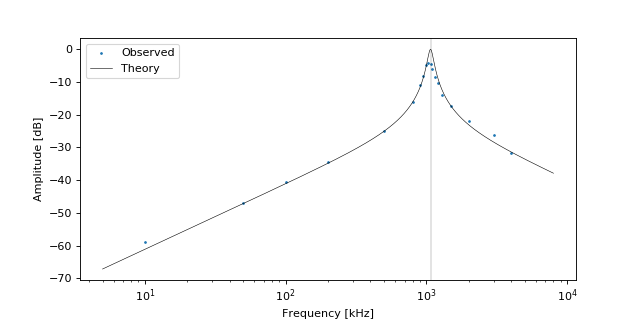
\includegraphics[width=12cm]{figures/series_resonant_RLC_amp.png}
        \caption{直列共振RLC回路の振幅応答}
    \end{center}
\end{figure}

また, 縦軸を位相として表示したものが以下である. 設計通り, 1MHz付近で位相が大きく動いていることが分かる. 
\begin{figure}[H]
    \begin{center}
     	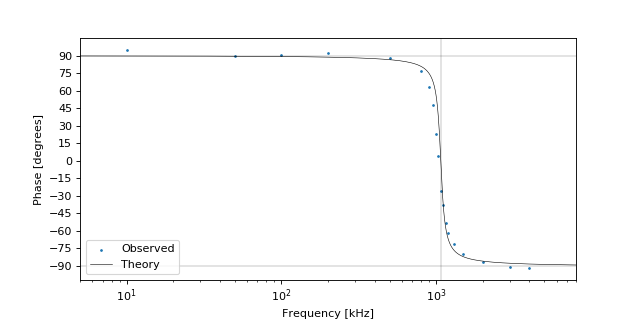
\includegraphics[width=12cm]{figures/series_resonant_RLC_phase.png}
        \caption{直列共振RLC回路の振幅応答}
    \end{center}
\end{figure}

(1)(b) 実験方法で述べた通りの方法で臨界的になる周波数を探した. 抵抗$R_0$を入れない場合の臨界値は$463\Omega$, 抵抗$R_0$を入れた場合の臨界値は$533\Omega$と計測された. また, ステップ応答は以下のようになった. 
\begin{figure}[H]
    \begin{center}
     	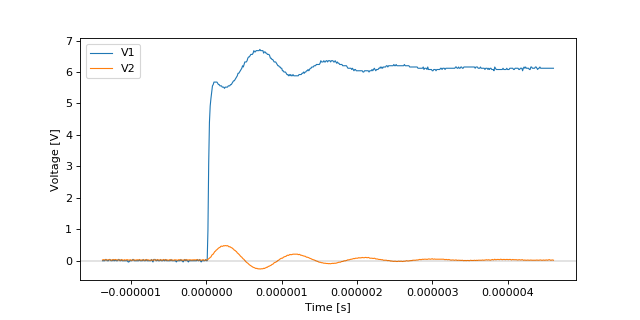
\includegraphics[width=12cm]{figures/1b.png}
        \caption{直列共振RLC回路の振幅応答}
    \end{center}
\end{figure}

\subsection{RC4端子網回路の測定}
(2)(a)こちらも同じく, 実験方法に書いた通りに測定した値を用い, 横軸を周波数, 縦軸を$V_2/V_1$のdB表示したものが以下のグラフである. 黒の実戦は使用した抵抗とキャパシタンスの値を用いて計算した理論値である. グラフから, 低周波数領域は通しており, また1213Hz付近から信号を通さなくなっていることが分かる. 


\begin{figure}[H]
    \begin{center}
     	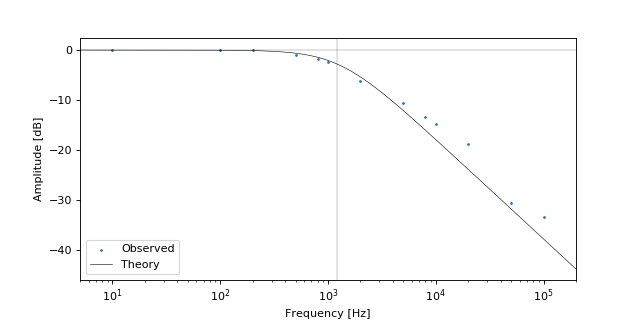
\includegraphics[width=12cm]{figures/four_terminal_RC_amp.png}
        \caption{RC4端子網回路の振幅応答}
    \end{center}
\end{figure}

また, 縦軸を位相として表示したものが以下である. こちらも, 1213Hzを中心に位相が変動していることが分かる. 


\begin{figure}[H]
    \begin{center}
     	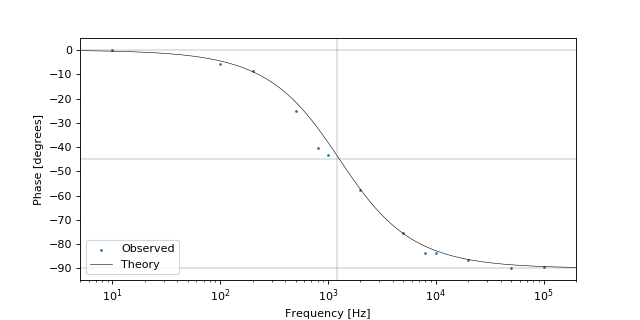
\includegraphics[width=12cm]{figures/four_terminal_RC_phase.png}
        \caption{RC4端子網回路の位相応答}
    \end{center}
\end{figure}

(2)(b)LPFに方形波を流し, 応答を見た. 
\begin{figure}[H]
    \begin{center}
     	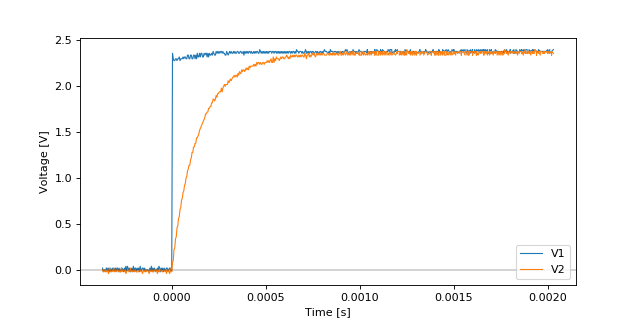
\includegraphics[width=12cm]{figures/2b.png}
        \caption{RC4端子網回路のステップ応答}
    \end{center}
\end{figure}

\section{考察課題}
(1)$v_1$を計測した場合, RLC回路の共振周波数付近ではファンクションジェネレーターの出力インピーダンスの$R_{out}$が大きくなるため, $R_{out}$での電圧降下を無視できなくなり, 正しい周波数特性を測定することができない. そこで, 図の$v_1$と$v_2$を測定する. ファンクションジェネレーターの出力インピーダンスを考慮すると, Yなどの値は以下となる. 
$$
Y=\frac{1}{R_{out} + R + sL + \frac{1}{sC}}
$$
ここで, 
$$
v_1 = \left(R+j(\omega L-\frac{1}{\omega C})\right)I
$$
$$
v_2 = RI
$$
であるため, 比をとると以下のようになる. 
$$
\frac{v_1}{v_2} = \frac{R}{R+j(\omega L-\frac{1}{\omega C})}
$$
この値は, $R_{out}$によって影響されない. $v_1$と$v_2$を計測することで, $R_{out}$によって影響されない周波数特性を求めることができる. \\

直列共振回路のアドミタンスは以下である. 
$$
Y(s) = \frac{1}{Z(s)} = \frac{1}{R+sL+\frac{1}{sC}} = \frac{s}{s^2L+sR+\frac{1}{C}}
$$
周波数特性は$s = j\omega$とおいて
$$
Y(j\omega) = \frac{1}{R+j\left(\omega L-\frac{1}{\omega C}\right)}
$$
となり, 大きさ, 偏角はそれぞれ

\begin{equation} \label{eq1}
\begin{split}
|Y(j\omega)| &= \left|\frac{1}{R+j(\omega L-\frac{1}{\omega C})}\right| \nonumber \\
&= \frac{1}{\sqrt{R^2+\left(\omega L-\frac{1}{\omega C}\right)^2}}\\
\mbox{arg} H(j\omega) &= tan^{-1}\frac{1}{R}\left(\frac{1}{\omega C}-\omega L\right)
\end{split}
\end{equation}

実験結果にその曲線を記した. 最大点は$\omega = \frac{1}{\sqrt{LC}}$で表される. 今回使用した素子の値を代入すると$\omega = \frac{1}{\sqrt{(47.3 \times 10^{-6})\times(467.4 \times 10^{-12})}} = 6.7255 \times 10^6$, 周波数に変換すると$f = 1.0704 \times 10^6$となる. 実験結果の図3において, 1.0704MHzのところに縦線を引いたが, 共振周波数が実験結果とよく一致していることが分かる. 実験で得られた最大値は$f=1030kHz$において-4.0dBであるため, 周波数の誤差は理論値の4\%程度である. 
\\Q値を求める. $Q = \frac{\omega}{\Delta\omega}$と表される. ここで, $\omega$はピーク時の値, $\Delta\omega$は電圧比の値が$1/\sqrt{2}$となるときの2つの周波数の差である. 実験結果のグラフに補助的な線を引いたものが以下である. ピーク値の$\frac{1}{\sqrt{2}}$の値ということは、ピーク時の値の$-3dB$であるため、$-4-3 = -7dB$のところに線を引き、実測値との交点の周波数を読み取った。

\begin{figure}[H]
    \begin{center}
     	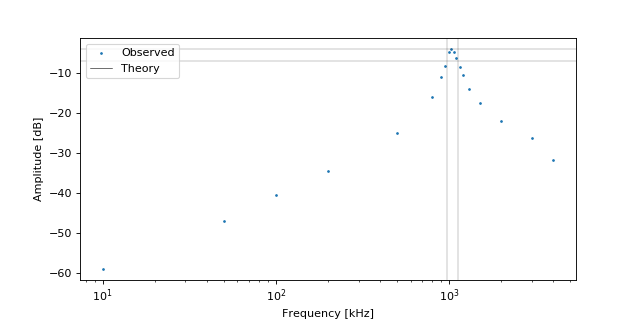
\includegraphics[width=12cm]{figures/series_resonant_RLC_amp_measure.png}
        \caption{RC4端子網回路の振幅応答}
    \end{center}
\end{figure}
ここから, 
$$\omega = 1040kHz,\, \omega_1 = 1120kHz,\, \omega_2 = 970kHz,\, Q = \frac{\omega}{\omega_1-\omega_2} = \frac{\omega}{\Delta\omega} = 6.93$$
と求まる. 実験に用いた素子を使ってQの値を計算すると
$$
Q = \frac{1}{\omega_0 CR} = \frac{1}{1030 \cdot 467.4 \times 10^{-12} \cdot 29.85} = 10.65
$$
となるため, 35\%の誤差率と分かる. \\

実測値から求めたQを用いて実効的なRの値を計算すると, $$R = \frac{1}{\omega_0 C Q} = 47.3$$となる. 使用した抵抗素子は$29.5\Omega$なので, 抵抗素子以外の部分での抵抗は$17.4\Omega$になると考えられる. インダクタの抵抗上限は$5.8\Omega$であるが, インダクタの抵抗が上限だったとしても25\%程度の誤差と分かる. \\

(2) (1)(b)において, ステップ応答が臨界的となったときの抵抗値を求める. \\
臨界的になる時, 
$$
\left(\frac{R}{2L}\right)^2 = \frac{1}{LC}
$$
$$
R = 2\sqrt{\frac{L}{C}} = 2\sqrt{\frac{47.3 \times 10^{-6}}{467.4 \times 10^{-12}}} = 636\Omega
$$
であると計算できる. ファンクションジェネレーターの出力インピーダンスは50$\Omega$なので, 可変抵抗の値は$636-29.9-50=556$となると分かる. オシロスコープを観測しながら可変抵抗の値を変え, 臨界的になる点を探した. 実測結果は$463\Omega$となった. これは誤差率が16.7\%である. \\

出力インピーダンスを下げる方法として, 抵抗$R_0$を挿入した. この結果, 等価な出力インピーダンスは$R_{out}$ではなく$1/(\frac{1}{R_{out}}+\frac{1}{R})$となる. また, RLC回路の実効的な抵抗成分は
$$
1/\left(\frac{1}{R_{out}}+\frac{1}{R_0}\right) + R = 1/\left(\frac{1}{50} + \frac{1}{4.69}\right) +R = 4.28 + R
$$
となり, 臨界点の可変抵抗の値は$636- 4.28 - 29.9 = 602$と計算できる. 実際に計測された値は$533\Omega$となったが, これの誤差率は11.5\%である. $R_0$を挿入する前と後の差は理論上$46\Omega$であるが, 実測値の差は$70\Omega$となっており, 想定される上がり幅よりも52\%ほど大きい上がり幅となった. \\~\\


(3) (2)(a)で測定した値を考察する. 伝達関数は
$$
H(j\omega) = \frac{1}{1+j\omega T}
$$
であるから振幅と位相は
$$
|H(j\omega)| = \left|\frac{1}{1+j\omega T}\right| = \frac{1}{\sqrt{1+\omega^2T^2}}
$$
$$
\mbox{arg} H(j\omega) = \mbox{tan}^{-1}(-\omega T)
$$
と求まる. この計算値を計測値とともにグラフに表示したものが実験結果のグラフである. 計測値と大まかな傾向は一致していることが分かる. 
1213Hzよりも大きなデータの部分を最小二乗法でフィッティングすると, 傾きが-0.857となった. 上の式を考えると, 高周波数域での伝達関数は$\frac{1}{sT}$と近似できる. その場合の両対数グラフの傾きは$-1$となるが, フィッティングした結果は理論値の86\%の値となっていることが分かる. 内部抵抗による誤差などは両対数グラフの傾きには影響しないと考えられるので, 実測された傾の方が絶対値が小さいのは他に原因があると考えられる. また, 位相特性は理論曲線とよく一致していることが分かる. \\~\\

(4)実験(1)(b)の結果のグラフのV1の値を計測用に拡大したものが以下である. 電圧をかけた直後の最大振幅は0.46V程度であり, その4\%の値は0.018Vである. グラフは0.02Vを中心としているため, $0.02V\pm 0.018V$のところに薄い 赤線を引いた. このような減衰振動では振動の振幅が4\%になるまでにほぼQ個の山が観測されるはずである. グラフから観測すると, この4\%に収まる前に少なくとも5個の山がある, ということが分かる. 考察(1)で実験値から求められたQの値は6.93であり, 4\%に収まるまでに実際には7個程度の山が観測されると予想できるが, データが$5.0\times 10^{-6}s$で切れており, これ以降のデータをとっていないことは反省すべき点である. 

\begin{figure}[H]
    \begin{center}
     	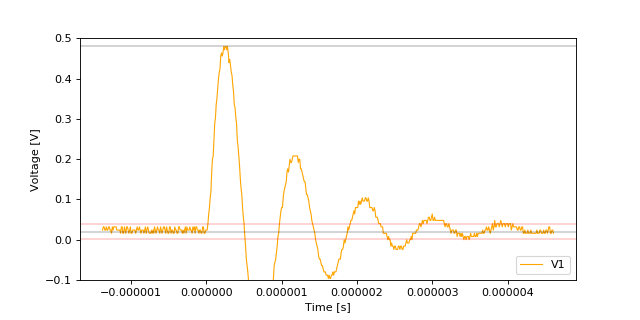
\includegraphics[width=12cm]{figures/1b(blownup).png}
        \caption{直列共振RLC回路の振幅応答}
    \end{center}
\end{figure}

(5)ステップ応答のT=0における微分係数は, 
$$
\frac{0.34 - (-0.02)}{2.0\times10^{-5} - 9.4\times10^{-12}} = 18000
$$
と計算できる. ステップ応答の最大値は2.36Vであり, 出力時の立ち上がりが経過時間に比例するため, 以下の式が成り立つ(ただしT=RCとする). 
$$
18000 = \frac{2.36}{T}
$$
$$
T = \frac {2.36}{18000} = 2.1 \times 10^{-4}
$$
ここで, しゃ断周波数$f_c$は$\omega T = 1$を満たすため, 
$$
f_c = \frac{1}{2\pi T} = 1213\mbox{Hz}
$$
であると計算できる. 一方, 実験の素子の値を用いて計算すると
$$
f_c = \frac{1}{2\pi T} = \frac{1}{2\pi \times 999 \times 124.9 \times 10^{-9}} = 1275 \mbox{Hz}
$$
であるので, 4.8\%の誤差であることが分かる. 実験結果の図には1213Hzの位置に線を引いた. 周波数特性は1213Hz付近で大きく減少していることが分かる. また, 位相についてであるが, しゃ断周波数付近では位相は\ang{-45}となるはずであるが, 実際に1213Hz付近で位相のずれが\ang{-45}となっている事がグラフからわかる. 

\section{参考文献} 
『ファンクションジェネレータの基礎と概要 (第1回)』\url{<https://www.techeyesonline.com/tech-column/detail/Reference-FunctionGenerator-01/?page=2>} 2021年4月10日アクセス\\

『Q値』\url{<http://ja.wikipedia.org/w/index.php?curid=47183>} 2021年4月11日アクセス\\

廣瀬 明. (2015). 電気電子計測[第2版]. 数理工学社

\end{document}



%-----------------------------------------------------------------------
%-----------------------------------------------------------------------Figu
%-----------------------------------------------------------------------
\begin{comment}
--見出し
\section{実験方法}
--番号を振る
\begin{enumerate}[label={(\arabic*)}]
\item
--画像の挿入
\begin{figure}[H]
    \begin{center}
     	\includegraphics[width=8cm]{figures/name}
        \caption{title)}
    \end{center}
\end{figure}

--回路(例)
\begin{figure}[H]
  \begin{center}
    \begin{circuitikz}[american currents]
     \ctikzset{american inductors}
	  \draw (0,0)
      to[sV=$V_s$] (0,2)
      to[L=$L_2$] (6,2)
      to[C=$$
      to[european resistor=$1\Omega$] (6,0)
      to[short] (3,0);
    \end{circuitikz}
    \caption{3次規格化0-R型LPF}
  \end{center}
\end{figure}

--表
\begin{table}[H]
    \begin{center}
        \begin{tabular}{|l|l|c||} \hline
            11 & 12 & 13 \\ \hline
            21 & 22 & 23 \\ \hline
            31 & 32 & 33\\ \hline
        \end{tabular}
        \caption{title}
    \end{center}
\end{table}
\end{comment}




























